\documentclass{article}
\usepackage[english]{babel}
\usepackage[utf8]{inputenc}
\usepackage{interval}
\usepackage{array}
\usepackage[table]{xcolor}
\usepackage{graphicx}
\usepackage{listings}
\usepackage{hyperref}
\usepackage{amssymb}
\usepackage{multicol}
\usepackage{amsmath, amsthm, amssymb, calrsfs, wasysym, verbatim, bbm, color, graphics, geometry}
\usepackage{graphicx}
\usepackage{float}
\usepackage{rotating}
\usepackage{adjustbox}
\usepackage{booktabs}
\usepackage{caption}
\usepackage{multicol}
\usepackage{amsmath}

\geometry{tmargin=.75in, bmargin=.75in, lmargin=.75in, rmargin = .75in} 

\DeclareMathOperator*{\argmax}{arg\,max}
\DeclareMathOperator{\EX}{\mathbb{E}}% expected value

\hypersetup{
	colorlinks,
	citecolor=black,
	filecolor=black,
	linkcolor=black,
	urlcolor=black
}
\DeclareUnicodeCharacter{2212}{-}
\begin{document}


\begin{titlepage}
      \centering
      \begin{figure}
            \begin{center}
                  
\includegraphics[width=0.6\textwidth]{img/UPM.png}
            \end{center}
      \end{figure}
      \vfill
      {\scshape\LARGE Image Processing, Analysis and Classification\\Academic Year 2023 \par}
      
      
      \vfill
      \newcommand{\HRule}{\rule{\linewidth}{0.3mm}}
      \centering
      \HRule \\[0.4cm]
      \huge  Clothing Co-Parsing with U-Net:\\
                a Semantic Segmentation journey\\% Title of your document
      \HRule \\
      \vspace{1cm}
      {\Large Sofia \textsc{Martellozzo}\par}
      {\Large(220894)\par}
      \vfill
      {\large Professor\par
          Jose \textsc{Crespo Del Arco}}
\end{titlepage}


\newpage
\renewcommand\contentsname{Contents}
\tableofcontents

\newpage

%------------------------------------------%
\section*{Overview}
The purpose of this project is to explore and learn about a computer vision topic.\\ 
In this case the research aims to explore more about semantic segmentation, specially in clothings images with the use of deep learning models.\\\\
The report starts from \ref{sec:introduction} an introduction of the topic, then \ref{sec:dataset} an overview over the dataset used. After that \ref{sec:architecture} an explanation on the architectures developed to save the task, how were trained and the results obtained \ref{sec:results}. In the last section \ref{sec:conclusions} the conclusions and some possible improvements.
%------------------------------------------%
\section{Introduction}\label{sec:introduction}
Semantic segmentation is a type of image segmentation that assigns a semantic label to each pixel in an image.\\
\begin{figure}[H]
    \begin{center}
    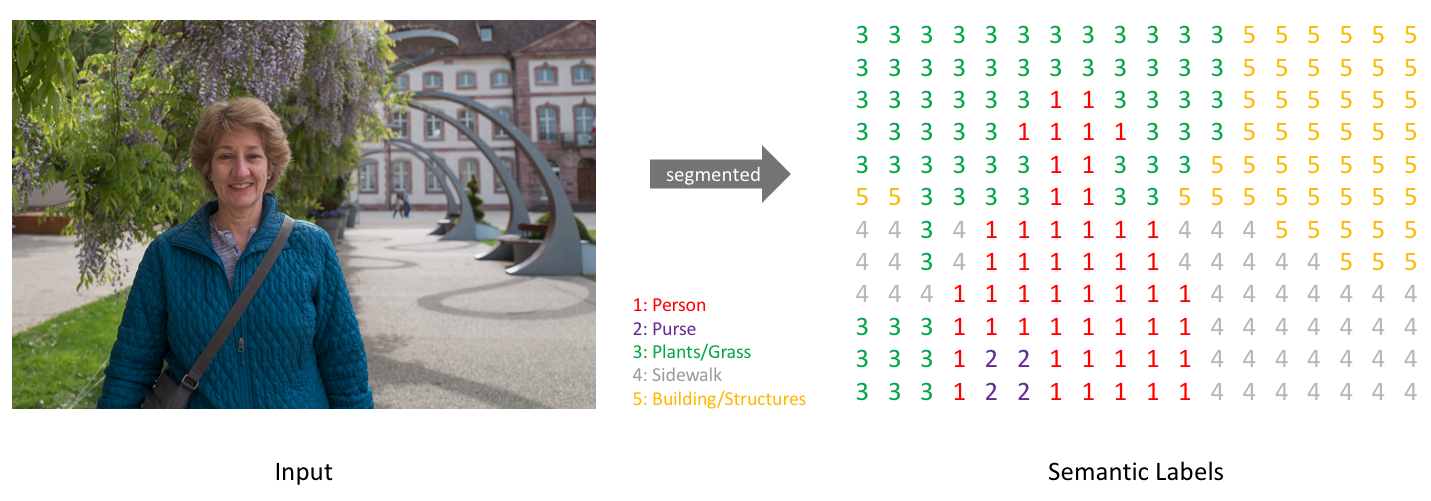
\includegraphics[width=0.4\textwidth]{img/SemanticSegmentation.png}
    \caption{Semantic Segmantation}
    \label{fig:semanticSegmentation}
    \end{center}
\end{figure}Unlike traditional image segmentation methods, which only consider low-level visual features such as color, texture, and brightness, semantic segmentation takes into account the context and meaning of the objects in the image. This means that pixels belonging to the same object or region are assigned the same label, even if they have different visual properties.\\
This allows the computer to understand the content of the image at a much deeper level than traditional segmentation techniques.
The process of semantic segmentation typically involves the use of deep neural networks, which output is a dense prediction mask, where each pixel is assigned a label corresponding to a particular object or region in the image.\\\\
Some common applications of semantic segmentation include:
\begin{enumerate}
    \item \begin{multicols}{2} Object recognition and detection: Semantic segmentation can be used to identify and locate objects in an image, which can then be used for tasks such as object recognition, tracking, and detection.\columnbreak 
    \begin{figure}[H]
        \begin{center}
        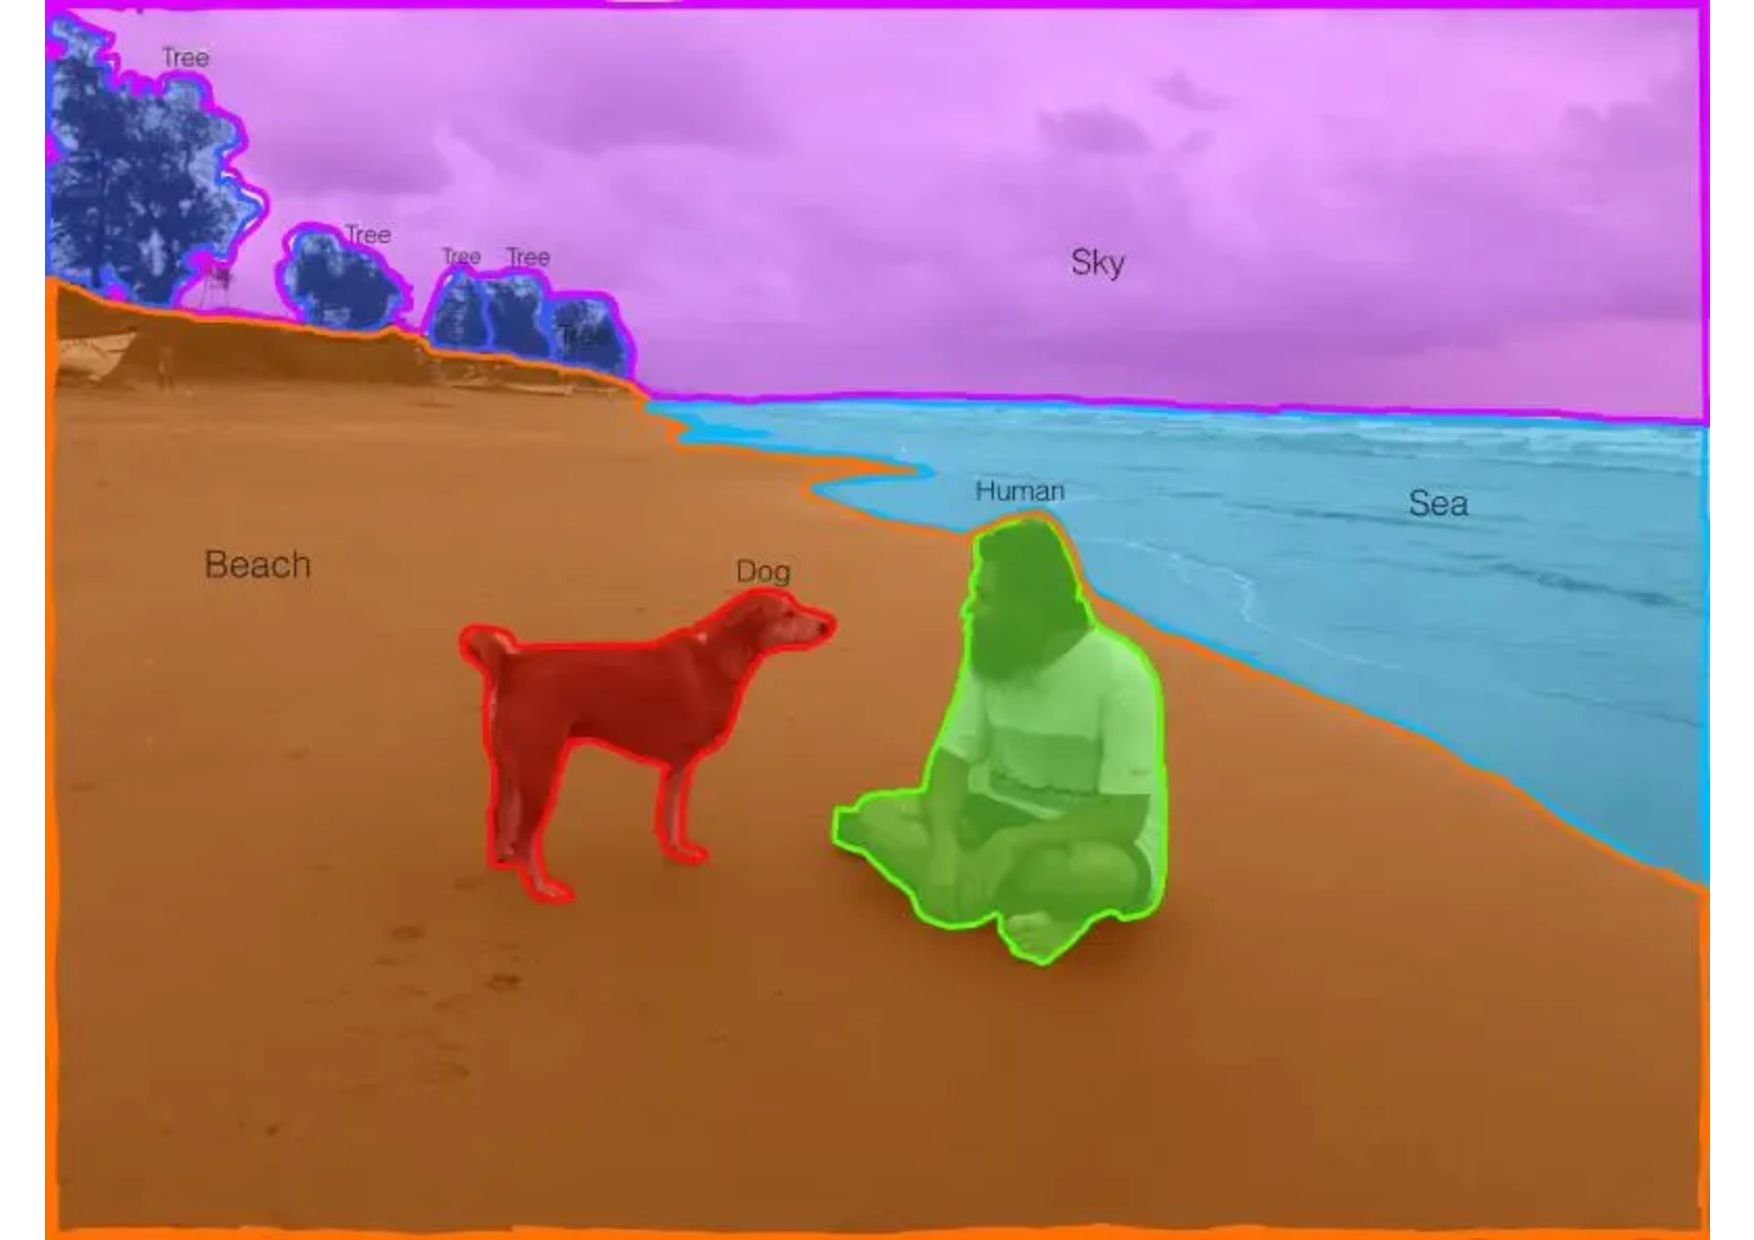
\includegraphics[width=0.18\textwidth]{img/ObjectRec.pdf}
        \label{fig:obgRec}
        \end{center}
    \end{figure}
    \end{multicols}
    \item \begin{multicols}{2} Scene understanding: Semantic segmentation can be used to understand the layout and composition of a scene, which can be useful for tasks such as autonomous navigation, virtual reality, and augmented reality.\columnbreak 
        \begin{figure}[H]
            \begin{center}
            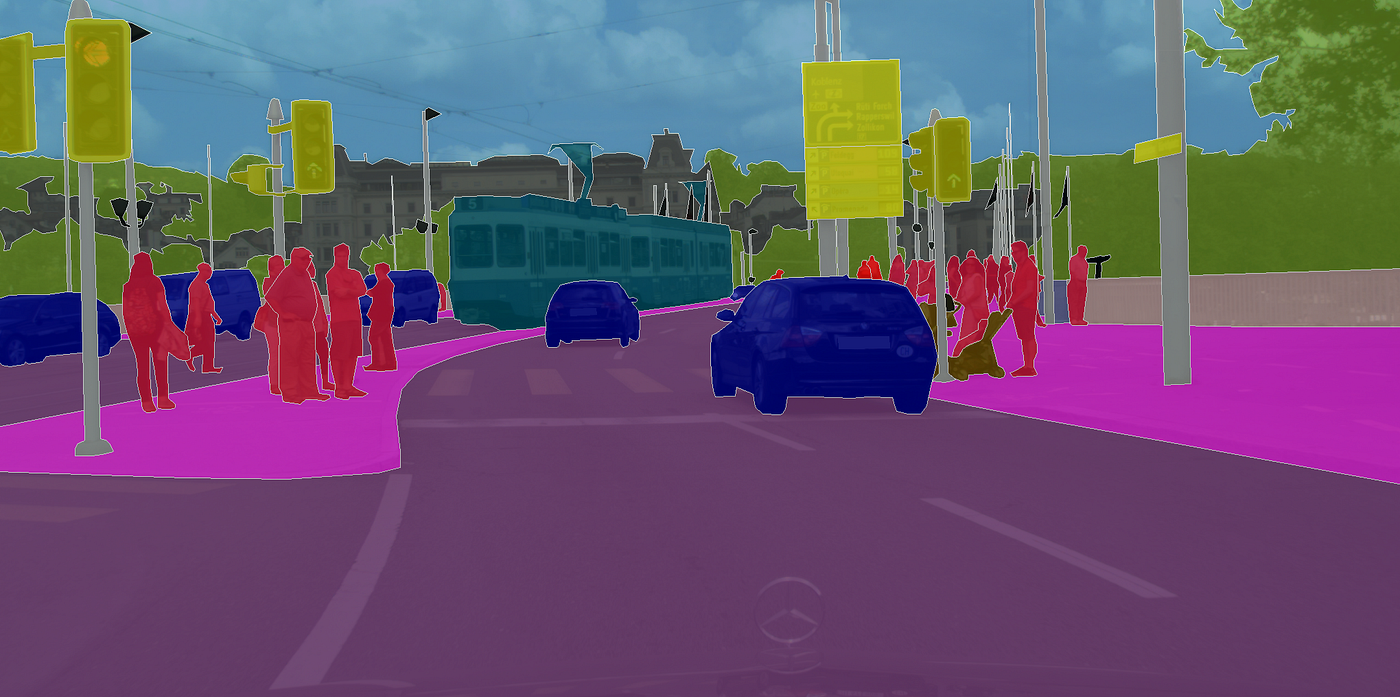
\includegraphics[width=0.2\textwidth]{img/SceneUnderstanding.png}
            \label{fig:scenUnd}
            \end{center}
        \end{figure}
    \end{multicols}
    \item \begin{multicols}{2} Image editing and manipulation: Semantic segmentation can be used to separate different objects or regions in an image, allowing for targeted editing and manipulation of specific parts of the image.\columnbreak 
        \begin{figure}[H]
            \begin{center}
            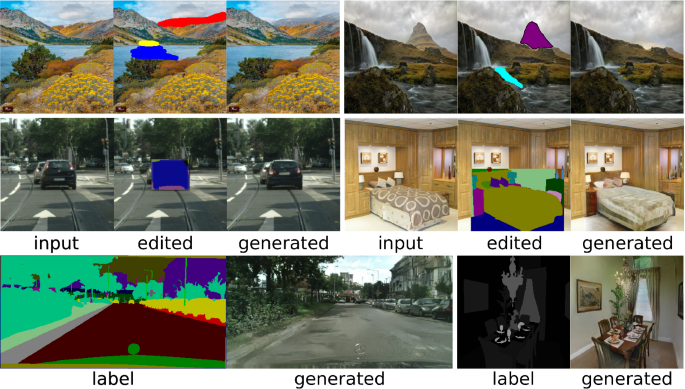
\includegraphics[width=0.28\textwidth]{img/ImageEditing.png}
            \label{fig:imgEdit}
            \end{center}
        \end{figure}
    \end{multicols}
\end{enumerate}
%------------------------------------------%
\section{Dataset}\label{sec:dataset}
The Clothing Co-Parsing (CCP) dataset is a collection of images of people.\\
The dataset contains over 20.000 samples, with a wide variety of clothing styles, poses and occlusions; and with pixel-level annotations for semantic segmentation of clothing items, such as pants, shirts and dresses.\\ The annotations were made by expert human annotators, ensuring high quality and accuracy.
It contains a total of 59 different labels.\\\\
The CCP dataset is a popular benchmark for semantic segmentation of clothing in computer vision research.\\ It has been used to develop and evaluate a wide range of algorithms for clothing parsing.
\begin{multicols}{4}
\begin{figure}[H]
    \begin{center}
    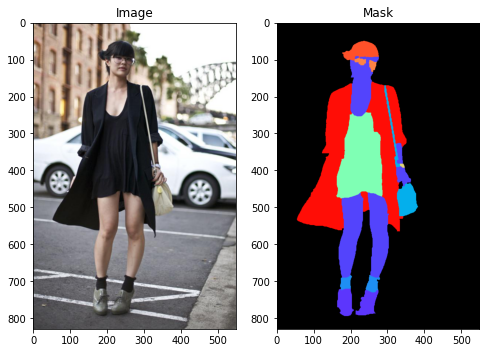
\includegraphics[width=0.25\textwidth]{img/FirstImMask.png}
    \label{fig:img1}
\end{center}
\end{figure}
\columnbreak
\begin{figure}[H]
    \begin{center}
    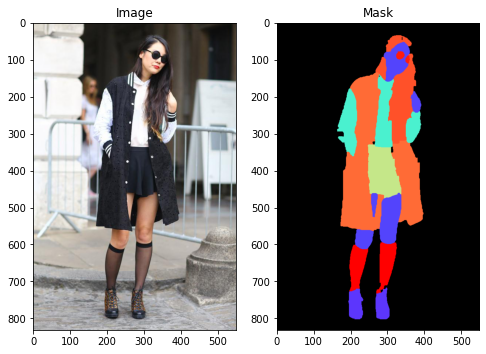
\includegraphics[width=0.25\textwidth]{img/SecondImMask.png}
    \label{fig:img2}
\end{center}
\end{figure}
\columnbreak
\begin{figure}[H]
    \begin{center}
    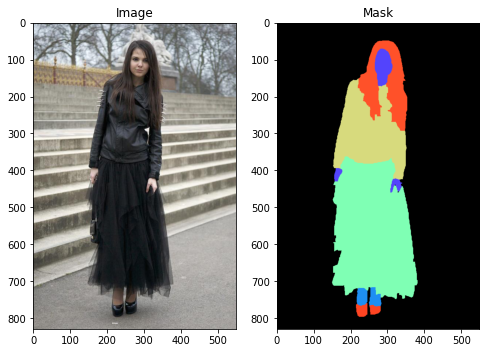
\includegraphics[width=0.25\textwidth]{img/ThirdImMask.png}
    \label{fig:img3}
\end{center}
\end{figure}
\columnbreak
\begin{figure}[H]
    \begin{center}
    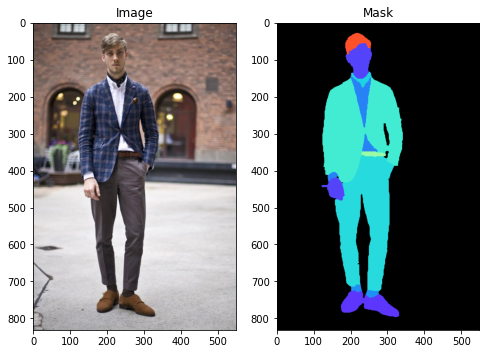
\includegraphics[width=0.25\textwidth]{img/FourthImMask.png}
    \label{fig:img4}
\end{center}
\end{figure}
\end{multicols}
\subsection{Pre-processing}
First of all the data has to be processed to fit properly with the model and to be all standardise, with same properties.\\
As previously mentioned, the dataset contains a large number of labels (59), including null (background), bag, belt, blazer, bodysuit, boots, and others.\\
However, the results of keeping all of these labels were not as good as expected. Therefore, to simplify the problem, the labels has been reduced to just 4, the most important components: the background, the clothes, the hair and the skin.
\begin{figure}[H]
    \begin{center}
    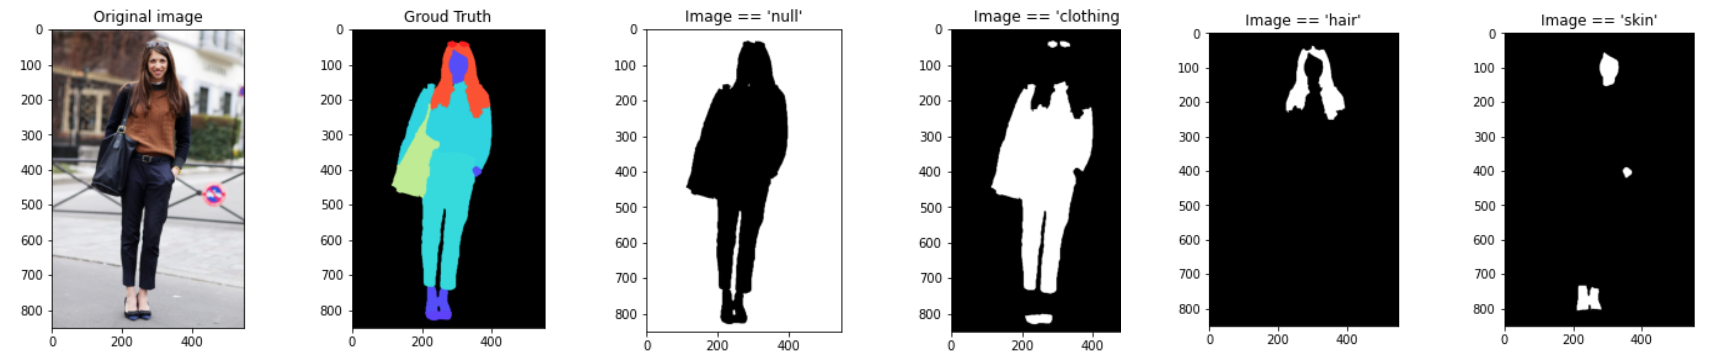
\includegraphics[width=0.8\textwidth]{img/4Components.png}
    \label{fig:4comp}
\end{center}
\end{figure}
The mask with the corresponding label for each pixel is modified accordingly.\\
The dataset has been devided in two groups: training and validation set, with a proportion of 90-10\% respectively. The choice of such an unbalanced division is the limited amount of data available in the dataset.\\ For this reason also data augmentation has been applied.\\\\
Data augmentation is a technique used in machine learning and deep learning to artificially increase the size and diversity of a training dataset. The goal of data augmentation is to improve the generalization and robustness of a model by exposing it to a wider range of input variations and perturbations.\\
Data augmentation involves applying a set of transformations to the original data, such as random rotations, translations, scaling, cropping, flipping, and color jittering, to generate new samples that are similar to the original data, but not identical.
By doing so, the model is exposed to variations and distortions that it might encounter in the real world, and is forced to learn more robust and invariant features.\\
Data augmentation is particularly useful in situations where the amount of available training data is limited, or where the data is highly imbalanced or biased. By generating new samples from the existing data, data augmentation can help to reduce overfitting and improve the generalization of the model.
The choice and magnitude of the transformations applied depends on the specific task and dataset, as well as the computational resources available.\\
In this case the transformations applied are:
\begin{itemize}
    \item Rotation of a range of 10
    \item Shift along height and weight of 10
    \item Horizontal flip
    \item Zoom of 30\% (just in one case, better explained later)
\end{itemize}
Finally a rescale operation of the training images has been performed by dividing all the pixel to 255 (that is the maximum possible pixel value). The purpose of rescaling an image in this way is to normalize the pixel values to a range between 0 and 1.\\
This is important because it ensures that all pixel values are on the same scale, which can be helpful for training machine learning models.By rescaling the image, it is also possible to reduce the computational resources required for processing the image, as the smaller pixel values require less memory and processing power.
%------------------------------------------%
\section{Architecture}\label{sec:architecture}
Semantic segmentation can be performed in different ways, with different deep learning model. The choice of the architecture end up in the U-Net architecture. The U-Net architecture follow the encoder-decoder architecture; It is composed of two main parts: the contraction path and the expansion path.
\begin{figure}[H]
        \begin{center}
        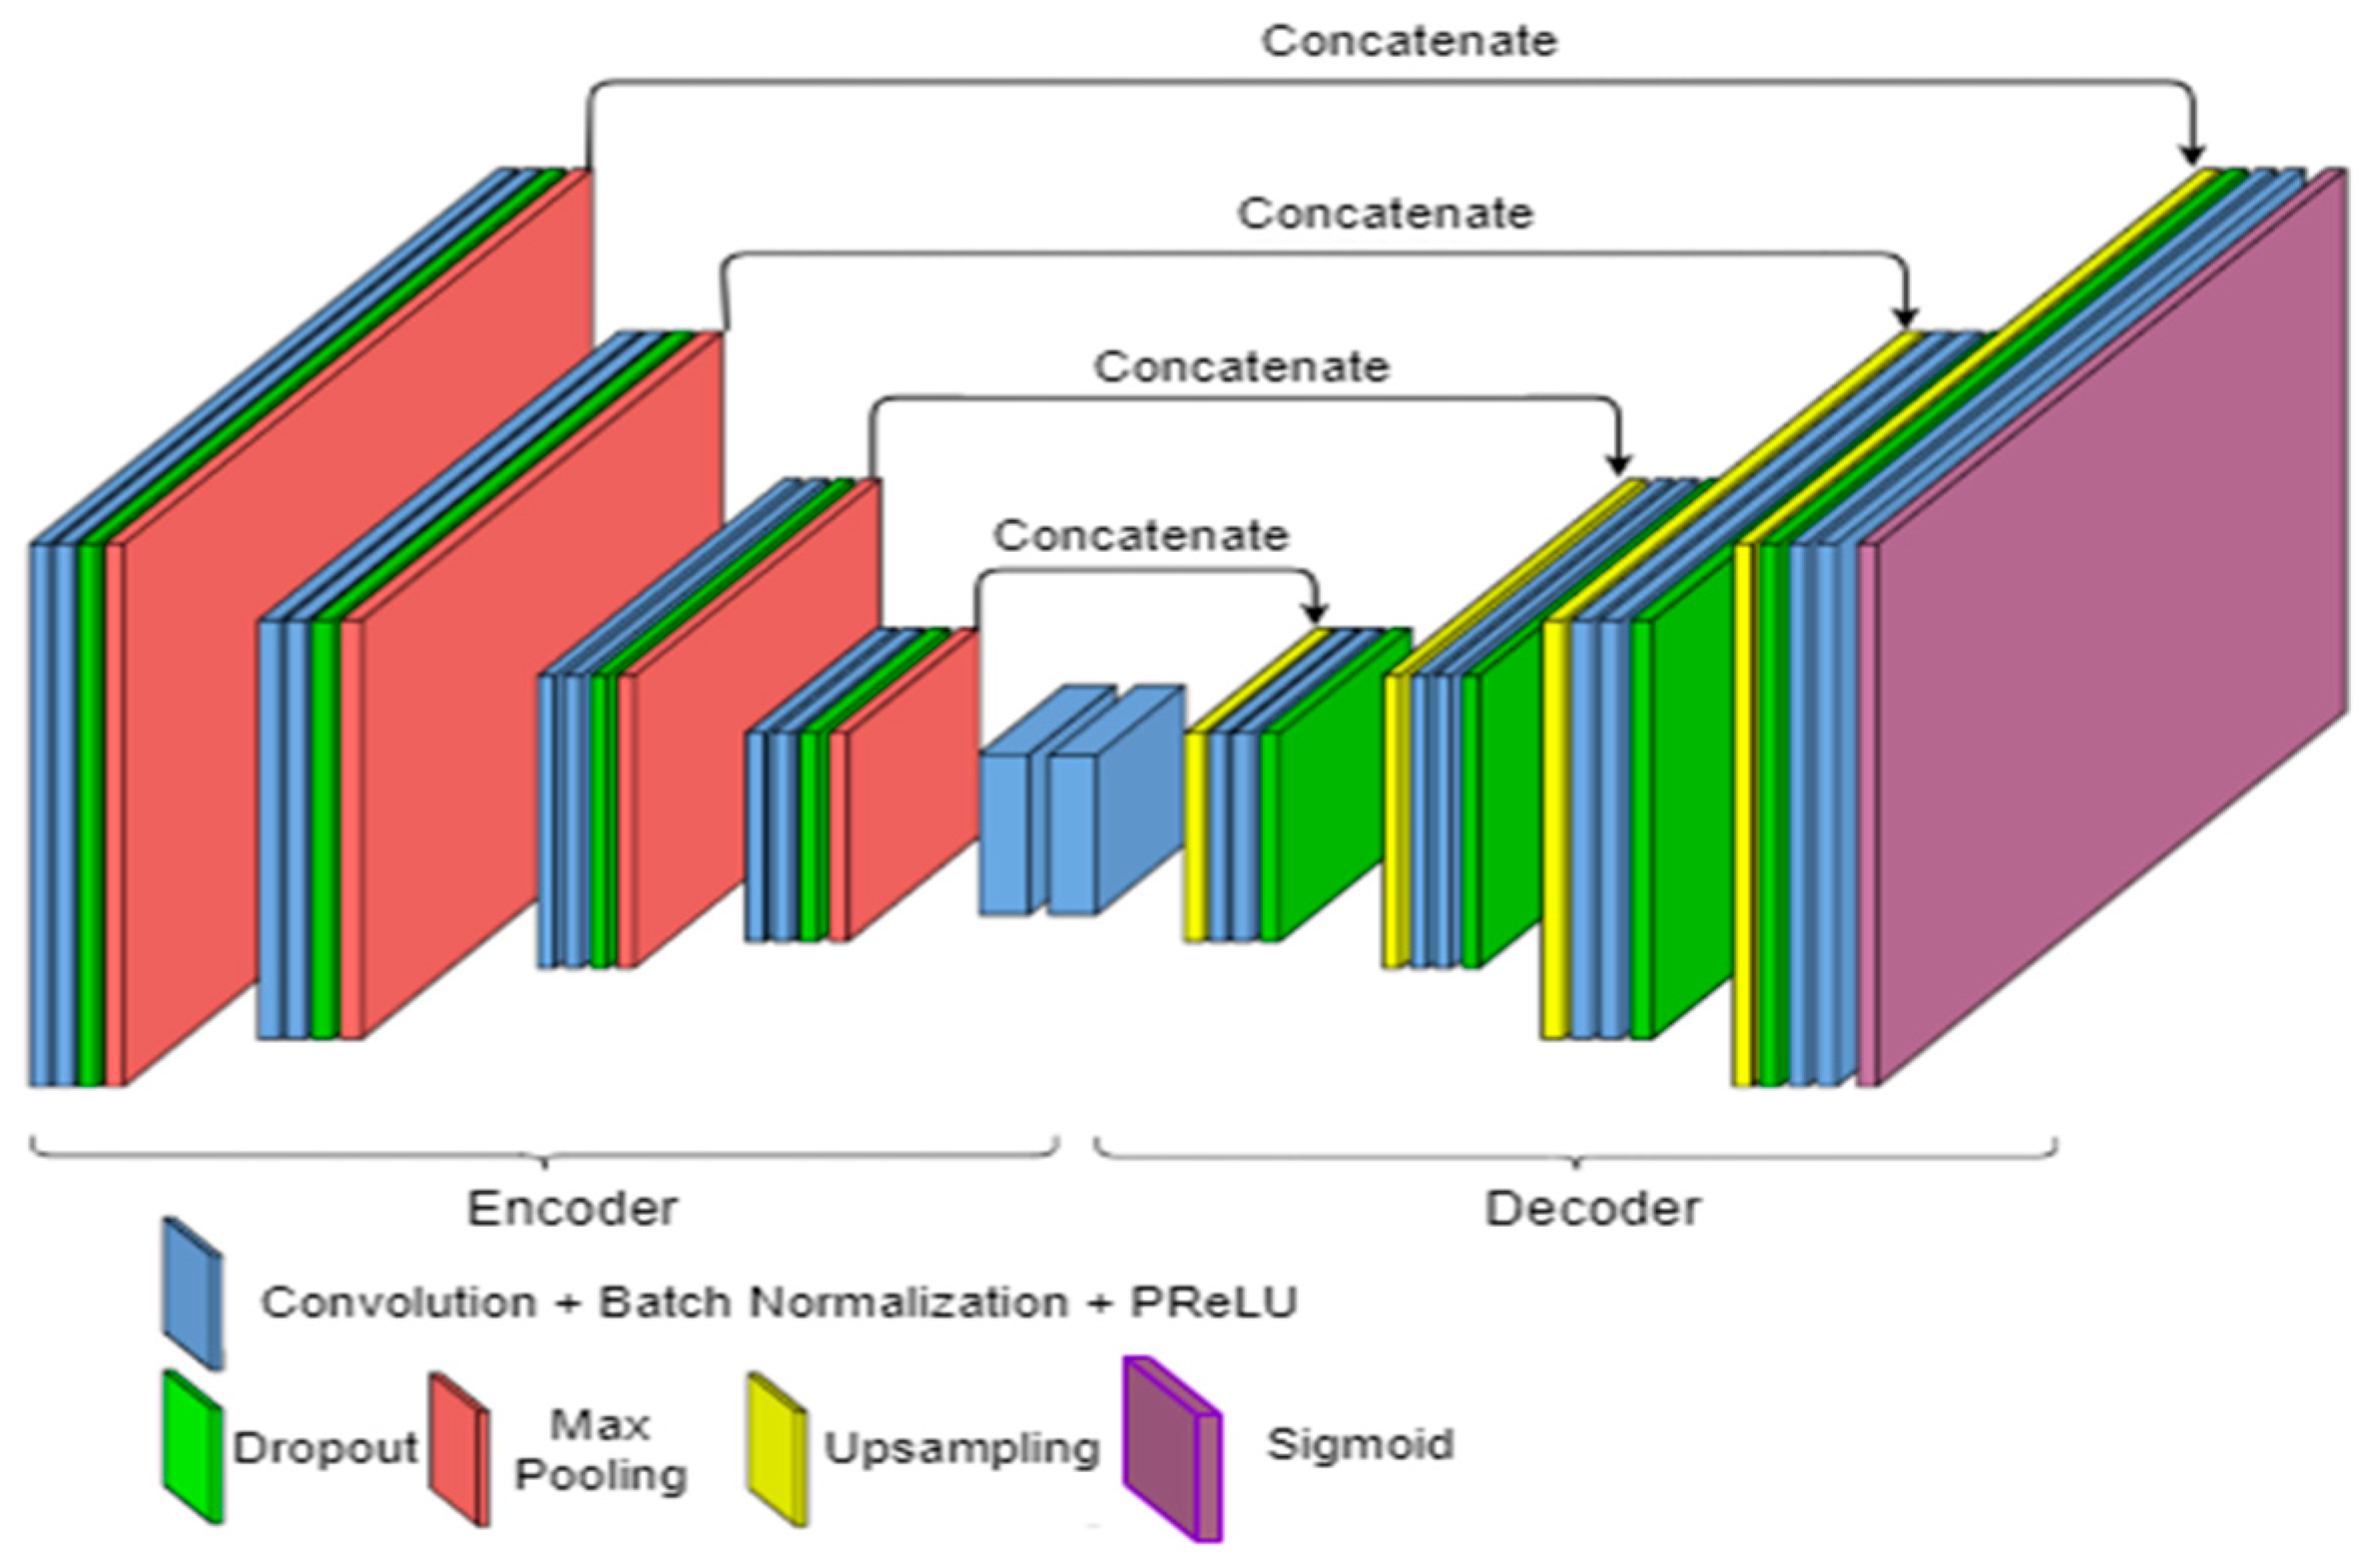
\includegraphics[width=0.3\textwidth]{img/U-Net.png}
        \caption{U-Net}
        \label{fig:unet}
    \end{center}
\end{figure} 
\begin{enumerate}
    \item The contraction path is similar to a typical CNN, where the input image is processed by a series of convolutional and pooling layers, to extract hierarchical features at different scales. This part of the network is responsible for capturing the context and spatial information of the input image.
    \item The expansion path is designed to recover the spatial resolution lost during the contraction path and produce the final segmentation map. The expansion path consists of a series of deconvolutional layers, which upsample the feature maps and combine them with the corresponding feature maps from the contraction path. This process allows the network to refine the segmentation boundaries and generate accurate segmentation masks.
    \item The U-Net architecture also incorporates skip connections between the contraction and expansion paths, which allow the network to fuse low-level and high-level features at different scales. These skip connections help the network to recover fine-grained details and improve the accuracy of segmentation.
\end{enumerate}
\subsection{Encoder}
The first part of the network is composed by a Convolutional Neural Network.\\
A CNN is a type of neural network that is commonly used in computer vision tasks, such as image classification, object detection, and image segmentation. It is designed to process input data with a grid-like structure, such as images, by learning a hierarchy of features at different spatial scales.\\
CNNs typically consist of multiple convolutional layers, interleaved with pooling layers, activation functions, and possibly other types of layers, such as dropout or batch normalization.
The combination of these layers allows the network to learn a hierarchy of increasingly complex features, from simple edges and textures to high-level object and scene representations.\\
\begin{multicols}{2}
    Convolutional layers are the basic building blocks of CNNs. A convolutional layer applies a set of filters, also known as kernels, to the input data and produces a set of feature maps as output. Each filter slides over the input data, performing a convolution operation between the filter weights and the input pixels at each location, producing a single output value. This operation is repeated for each location in the input data, producing a feature map. Convolutional layers are designed to capture local spatial patterns in the input data, such as edges, corners, and textures\columnbreak
    A pooling layer is a type of layer in a neural network used for down-sampling or reducing the spatial dimensions (height and width) of feature maps produced by a convolutional layer. The pooling operation involves dividing the feature map into non-overlapping sub-regions or windows, and then applying a pooling function, such as max pooling or average pooling, to each sub-region. The output of the pooling operation is a down-sampled feature map with reduced spatial dimensions but retaining the important features of the original feature map. The pooling layer helps to reduce the number of parameters in the network and prevent overfitting, while also increasing computational efficiency.
\end{multicols}
\begin{multicols}{2}
    \begin{figure}[H]
        \begin{center}
        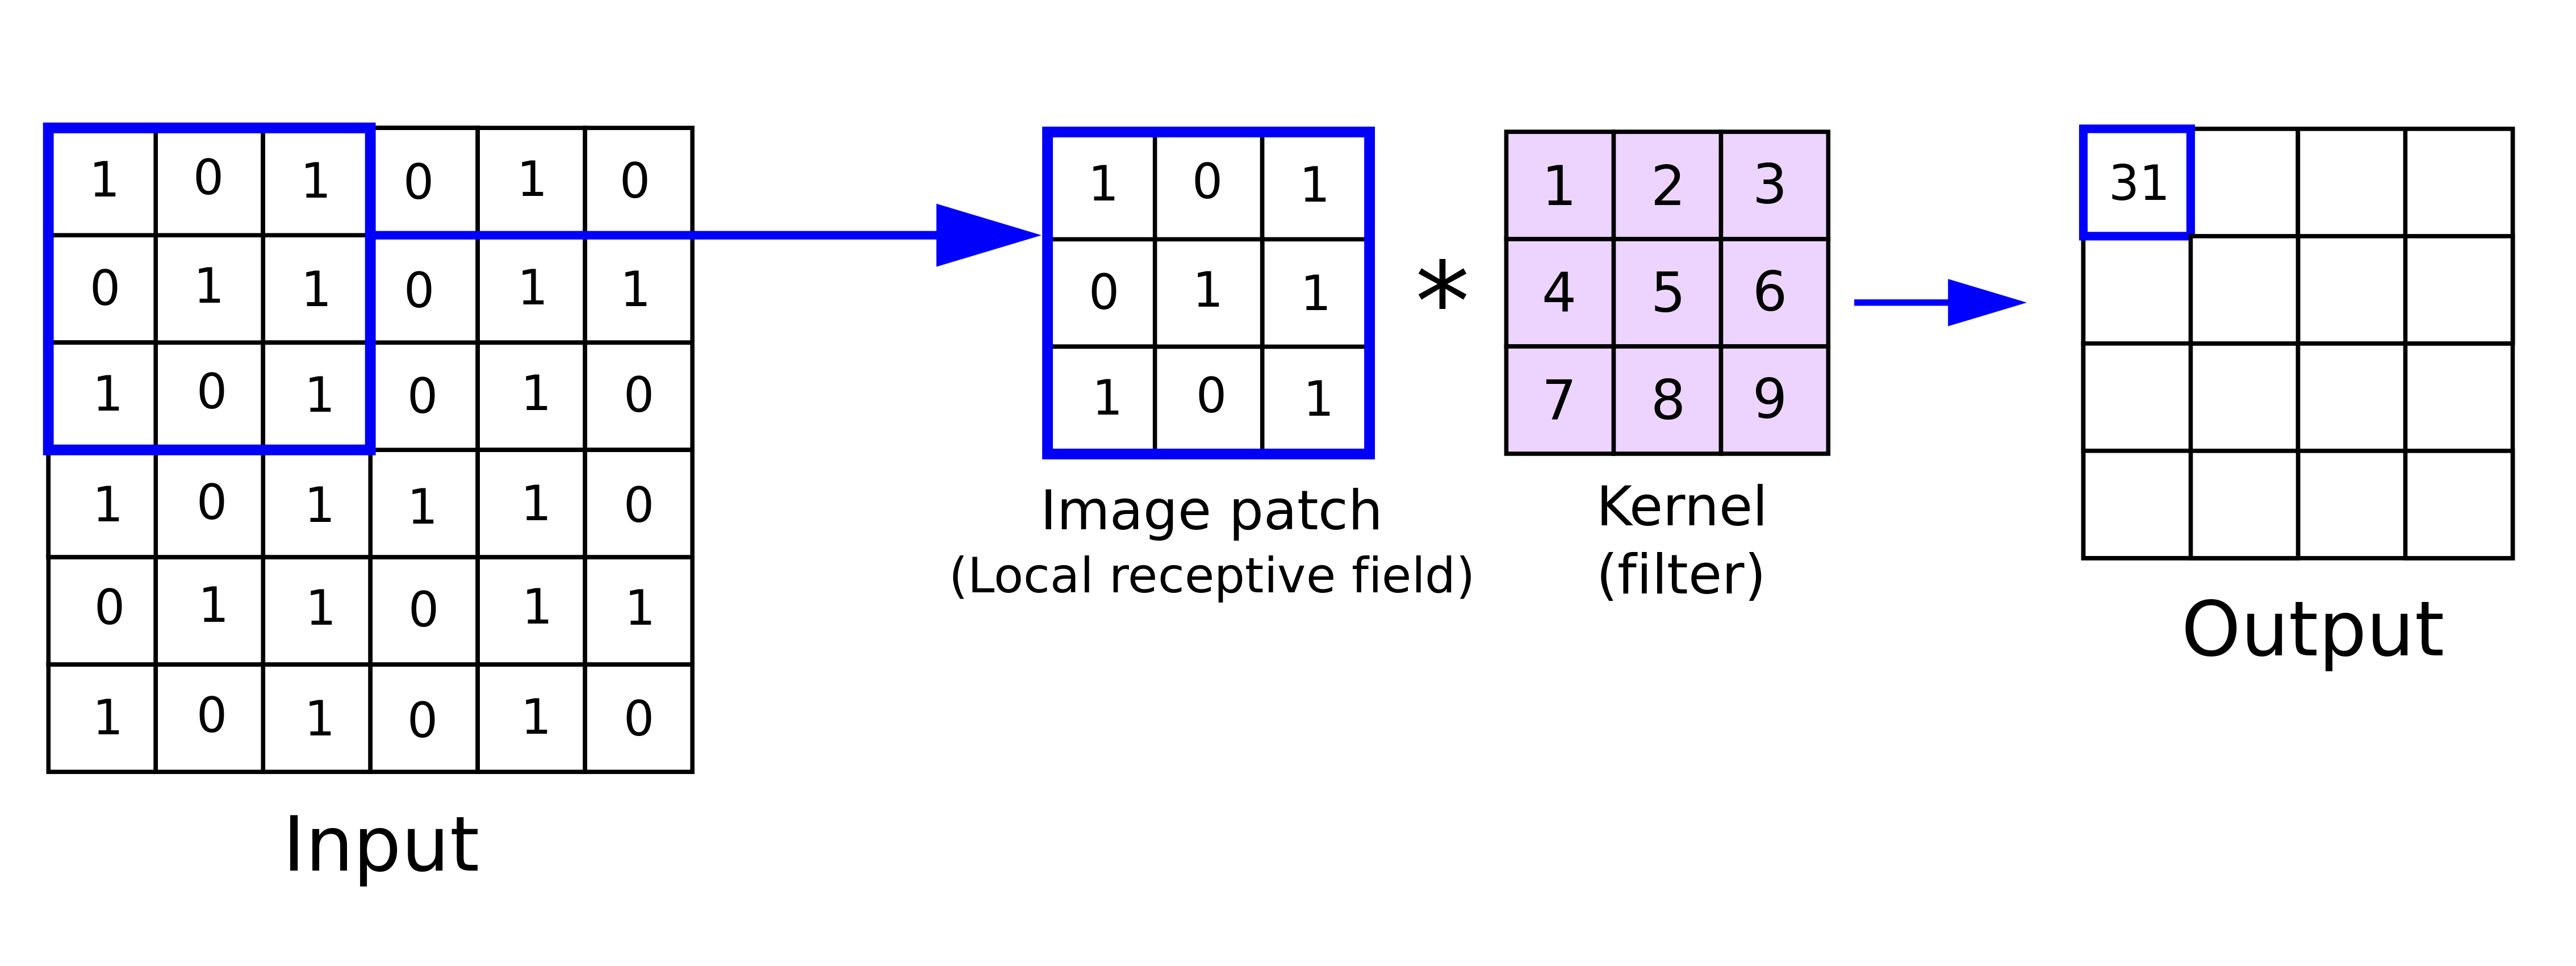
\includegraphics[width=0.25\textwidth]{img/convLayer.png}
        \caption{Convolutional layer}
        \label{fig:convL}
    \end{center}
\end{figure}
    \columnbreak
    \begin{figure}[H]
        \begin{center}
        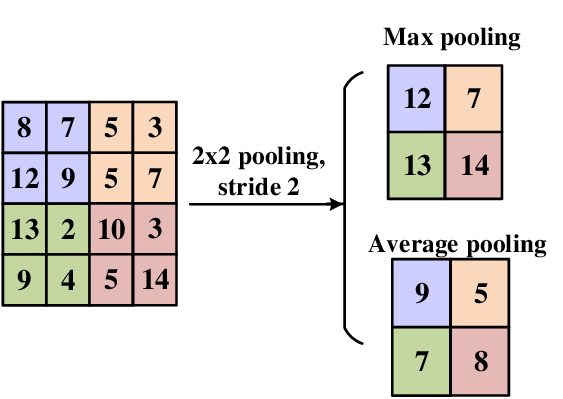
\includegraphics[width=0.2\textwidth]{img/poolingLayer.png}
        \caption{Pooling Layer}
        \label{fig:poolL}
    \end{center}
\end{figure}
\end{multicols}
For the first part of the architecture (the encoder) the convolutional neural network chosen are two known, downloaded from eras library: VGG16 and VGG19. The two models are downloaded without their weights, no transfer learning performed, setting all theirs layers trainable and removing their top, the last layers in order to perform just the feature extraction.
\subsection{Decoder}
On the other hand, at the second part of the architecture, to perform the segmentation, many upooling and deconvolution layers are attached. Upooling and deconvolution layers are two types of layers are used to increase the spatial resolution of feature maps, which is often necessary to generate more accurate and detailed segmentation maps.
\begin{multicols}{2}
    Unpooling layers are used to reverse the pooling operation. 
Pooling is used to downsample the feature maps and increase the receptive field of the network, but it also causes a loss of spatial information. 
Unpooling layers are used to recover this lost information and restore the original spatial resolution of the feature maps. Unpooling can be performed in various ways, such as by storing the locations of the maximum values during the pooling operation and using them to place the values back in the correct locations during unpooling. Alternatively, unpooling can be performed using interpolation techniques, such as nearest neighbor or bilinear interpolation, to fill in the missing values.\columnbreak
Deconvolution layers, also known as convolutional transpose layers, are often used in combination with unpooling layers to perform upsampling and restore the original spatial resolution of feature maps. Deconvolution layers use a set of learnable filters to generate new features from the existing ones, and can be used to perform upsampling in a learnable manner. However, they can also introduce artifacts and distortions if not used carefully.
\end{multicols}
\begin{multicols}{2}
    \begin{figure}[H]
        \begin{center}
        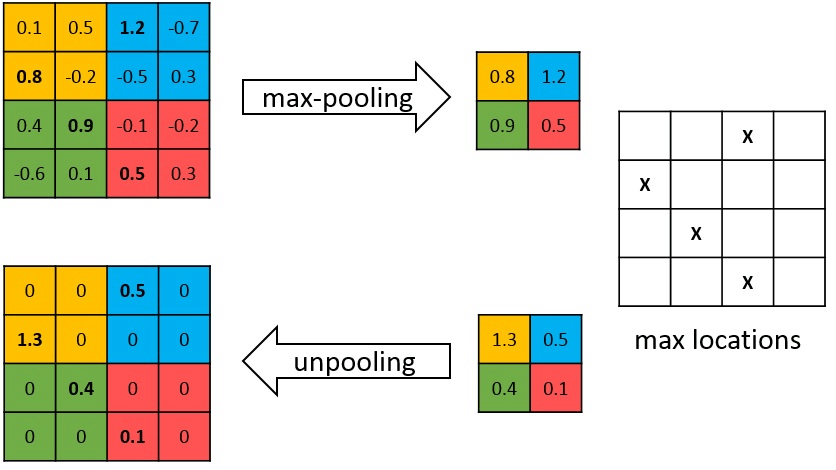
\includegraphics[width=0.25\textwidth]{img/unpoolingLayer.png}
        \caption{Unpooling Layer}
        \label{fig:unpoolL}
    \end{center}
\end{figure}
    \columnbreak
    \begin{figure}[H]
        \begin{center}
        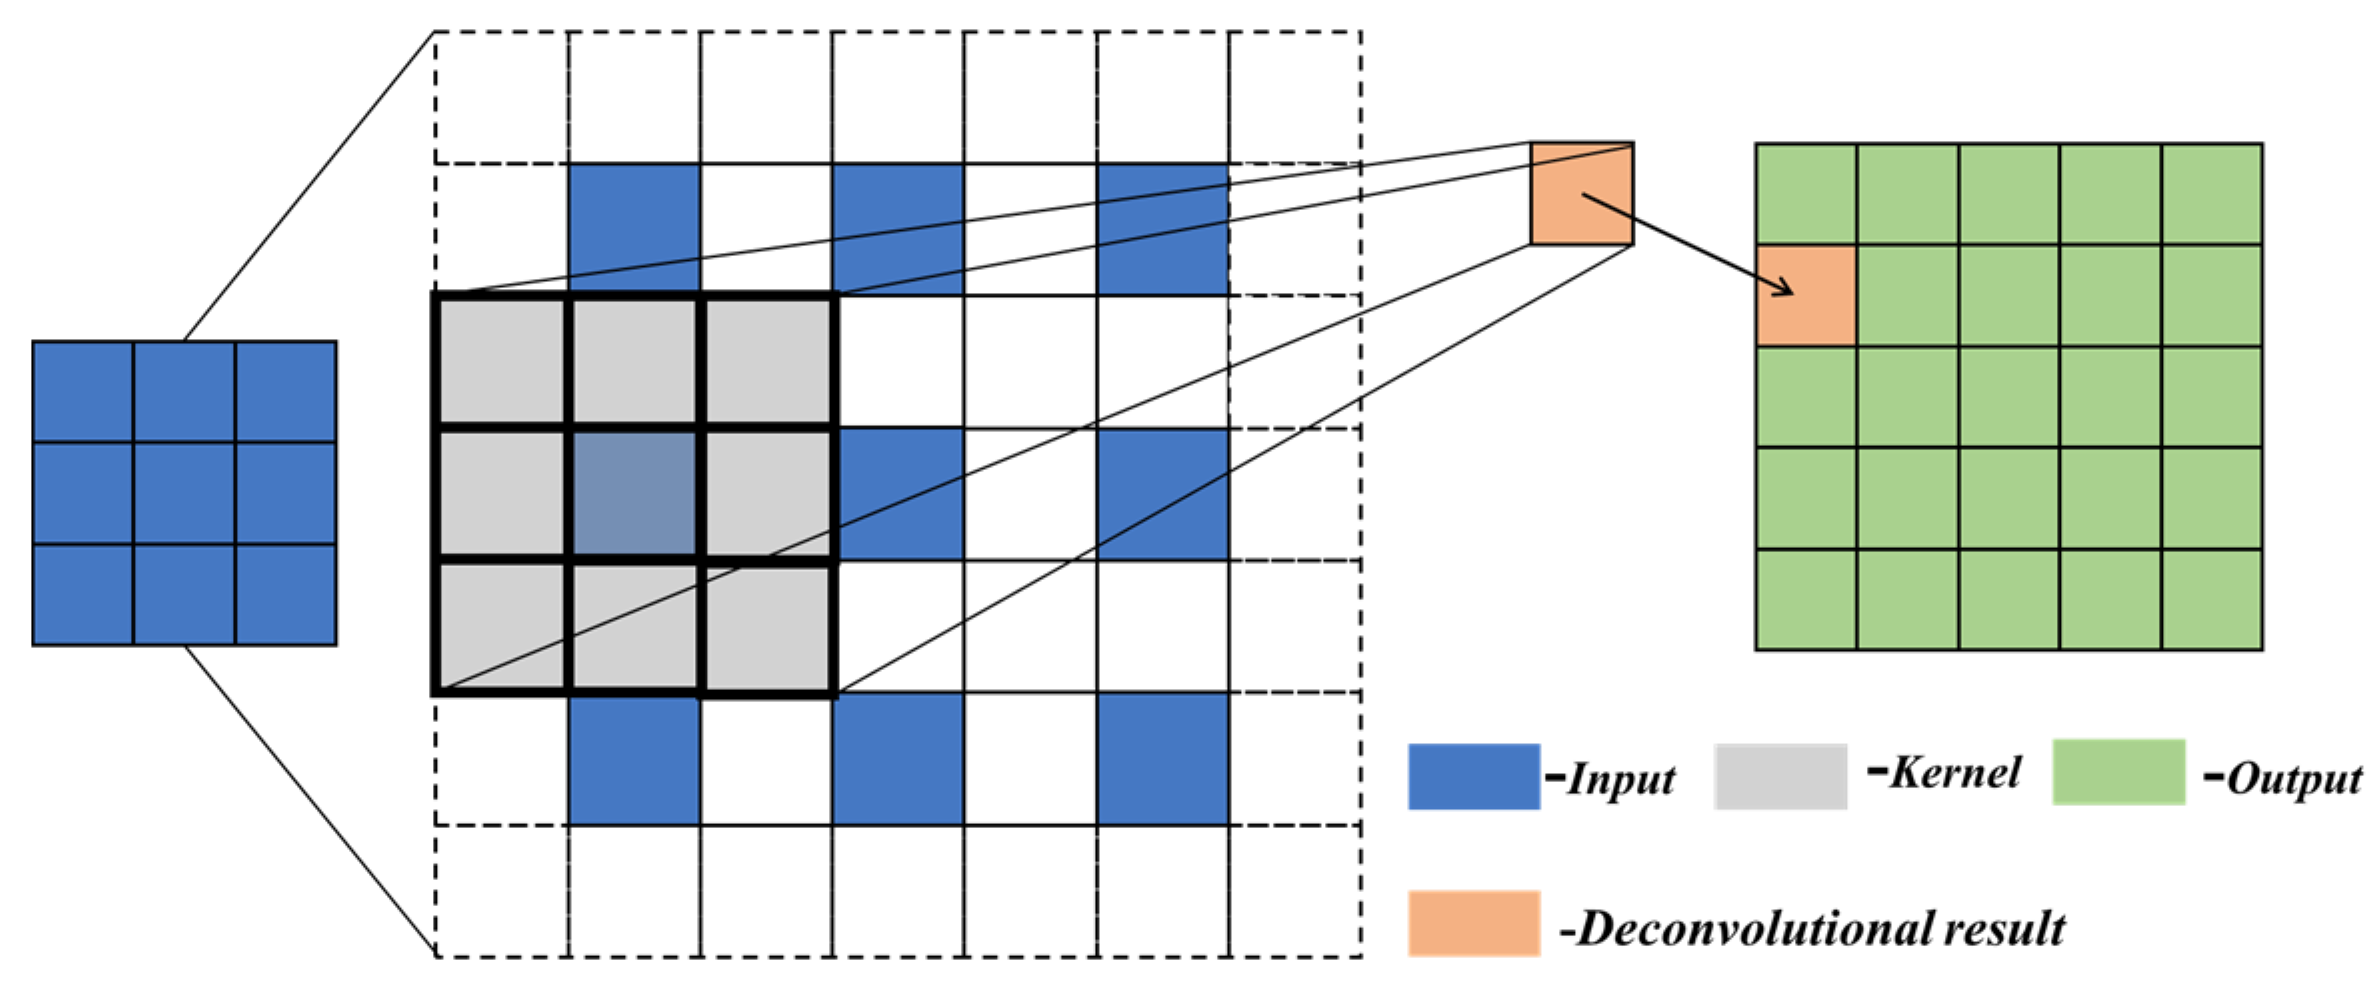
\includegraphics[width=0.2\textwidth]{img/deconvolutionLayer.png}
        \caption{Deconvolution Layer}
        \label{fig:deconL}
    \end{center}
\end{figure}
\end{multicols}
\subsection{Skip connection}
Skip connection is a type of shortcut connection that allows information to be passed directly between non-adjacent layers in a neural network. Specifically, a skip connection connects the output of a layer to the input of a layer that is not directly adjacent to it, typically one or more layers further down the network. The output of  layer is added to the input of a non directly adjacent layer.  By allowing information to bypass several layers at once, skip connections can help to preserve important information and gradients that might otherwise be lost as they propagate through the network.\\\\
The operation seen till now are used to increase the receptive field of the network and extract increasingly abstract features, but they also result in a loss of spatial information and can make it difficult to accurately localize object boundaries.
Skip connections are a way to address this problem by preserving information from the earlier stages of the network and combining it with information from the later stages. Skip connections allow the network to capture both high-level semantic information and low-level spatial information, and to fuse them together to address the challenge of accurately localising object boundaries and preserving fine-grained details, creating a more accurate segmentation map.  
%------------------------------------------%
\section{Training and Results}\label{sec:results}
The training setting are composed by a number of epochs equal to 100, even if all of the trials no more than 30 epochs were needed. To overcome the overfitting problem, early stopping has been adopted.\\
Early stopping is a technique to monitor the training and the validation error during the training to detect when the model is overfitting and stop the execution. A patience of 5 is set for the early stopping parameter, that is the number of epochs with no improvement after which training will be stopped.\\
Adam has been chosen as optimiser, with learning rate of 0.0001 and a batch size of 8 elements.
\subsection{Results}
The first trial is with VGG16 as backbone of the U-Net and by including all 59 different labels present in the dataset.\\The first image shows the original input to the network, while the second image displays the true mask with a different color assigned to each label. The third image shows the output predicted by my model.\\Despite the low expectations, the model was able to detect most of the important parts. However, the predictions are not very precise and sometimes mistakenly classify parts of the background as something else. This is because the model was searching for more detailed distinctions among the labels.
\begin{figure}[H]
    \begin{center}
    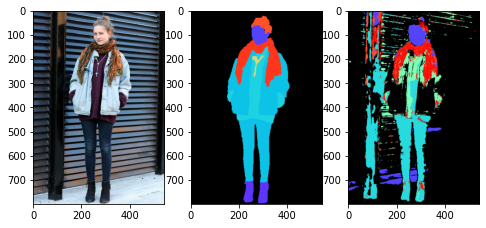
\includegraphics[width=0.4\textwidth]{img/FirstResult2.png}
    \label{fig:res1}
\end{center}
\end{figure}
\begin{multicols}{3}
The second trial with still the VGG16 but just 4 labels detect better the contours of the figure in the image, but is not properly able to distinguish between clothes, skin and hair.\\
\columnbreak
The other CNN (the VGG19) performs better achieving the following result.In this case the difference between clothes and skin is found but in most of the case it struggle in detecting the pixels containing the hair, since is a way more restricted part.\\
\columnbreak
For the first 3 trials, during data augmentation, the zooming transformation were not performed. As last trial it is added achieving results even a little bit worse, but not in a very significant way.
\end{multicols}


\begin{multicols}{3}
    \begin{figure}[H]
        \begin{center}
        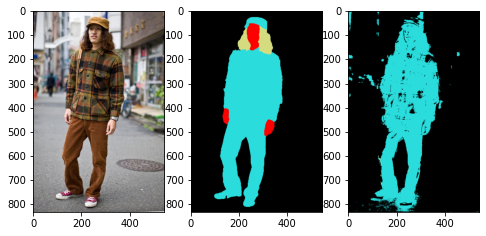
\includegraphics[width=0.3\textwidth]{img/SecondResult.png}
        \label{fig:res2}
    \end{center}
    \end{figure}
    \columnbreak
    \begin{figure}[H]
        \begin{center}
        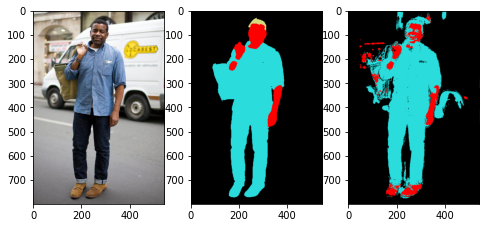
\includegraphics[width=0.3\textwidth]{img/ThirdResult.png}
        \label{fig:res3}
    \end{center}
    \end{figure}
    \columnbreak
    \begin{figure}[H]
        \begin{center}
        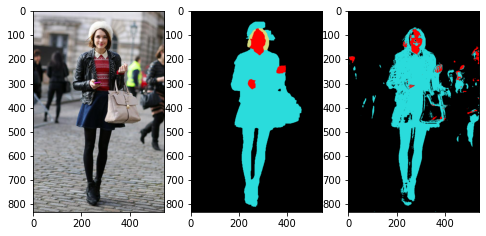
\includegraphics[width=0.3\textwidth]{img/FourthResult.png}
        \label{fig:res4}
    \end{center}
    \end{figure}
\end{multicols}
%------------------------------------------%
\section{Conclusions}\label{sec:conclusions}
In conclusion, a U-Net model has been developed for semantic segmentation of the Clothing Co-Parsing dataset, which has shown promising results. 
U-Net is a powerful and effective architecture for image segmentation, with state-of-the-art performance on many benchmark datasets. Its simple yet elegant design and ability to handle small datasets make it a popular choice for many researchers and developers working on image segmentation tasks.\\
Although the model's performance is good, there is still room for improvement: 
\begin{itemize}
    \item One possible idea could be to use more data, for example as done on the paper(link) found about this topic, in which the developer combined the CCP dataset with another one, Colourful Fashion Parsing (CFPD). The quality and size of the training dataset can greatly impact the model's performance.
    \item Other types of augmentation technique or combination of them could improve the performance of the model as well. Some of them were used here, with always the same parameters or adding the zoom effect, since each trial requires to retrain the hole network that is time consuming and also require a lot of resources.
    \item Moreover, optimizing the model's hyperparameters, such as learning rate and regularization, can also help improve the model's performance. 
    \item Additionally, experimenting with different Convolutional neural network can be considered such as: ResNet, efficientNet.
    \item Or also with another architecture different from U-Net, in the paper(link) there were mentioned Linknet, Pspnet, Fpn.
\end{itemize}

\newpage
%------------------------------------------%
\section*{References}
{[0]}Andrei de Souza Inácio, Anderson Brilhador, Heitor Silvério Lopes. Semantic segmentation of clothes in the context of soft biometrics using deep learning methods.\\
{[1]}\href{https://github.com/bearpaw/clothing-co-parsing}{Dataset}\\
{[2]}\href{https://github.com/mberkay0/clothing-segmentation}{Clothes Segmentation using DeepLabV3+}\\
{[3]}\href{https://keras.io/api/applications/vgg/}{Keras VGG16 and VGG19}

\end{document}